\block{5. Structural Embedding: Coalition vs.\ Opposition}{
    \centering
    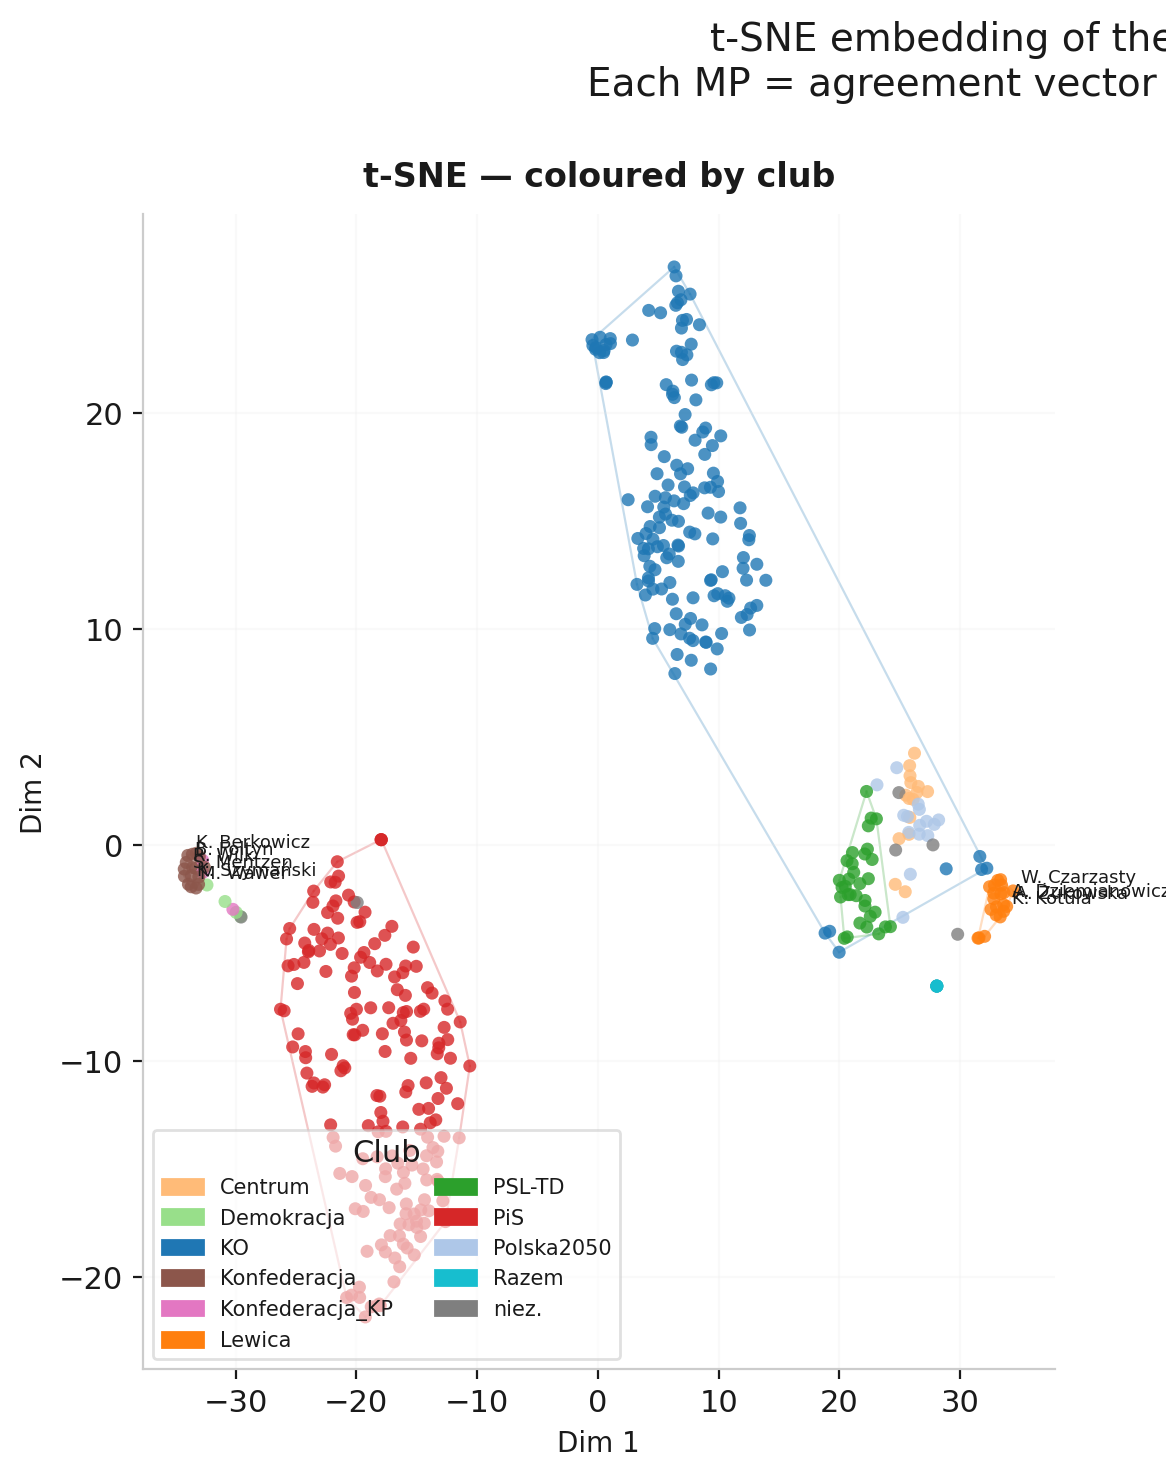
\includegraphics[height=24cm]{fig32_club_only.png}
    \vspace{0.3cm}

    \flushleft
    \textbf{Method:} t-SNE applied to the raw voting agreement vectors of all 459 MPs — \emph{no party labels used during embedding}.

    \vspace{0.4cm}
    \textbf{Key Findings:}
    \begin{itemize}
        \item \textbf{Self-organisation:} MPs cluster by party purely from voting behaviour, confirming that ideological affiliation is the dominant driver of parliamentary decisions.
        \item \textbf{Clear Divide:} Coalition (red) and opposition (dark) separate with a Silhouette score of \textbf{0.680} — a strong and statistically significant split.
        \item \textbf{Bridge MPs:} A small set of independents and \textit{Demokracja} MPs appear in the border zone, acting as potential cross-bloc mediators.
    \end{itemize}
}